\documentclass[11pt,a4paper]{article}

%% ── packages ──────────────────────────────────────────────────────
\usepackage[utf8]{inputenc}
\usepackage[T1]{fontenc}
\usepackage{microtype}
\usepackage{geometry}
\geometry{margin=2.4cm}
\usepackage{booktabs,array}
\usepackage{graphicx}
\usepackage{xcolor}
\usepackage{hyperref}
\usepackage{enumitem}
\usepackage{caption}
\usepackage{subcaption}
\usepackage{amsmath,amssymb}
\usepackage{setspace}
\usepackage{parskip}

%% ── metadata ──────────────────────────────────────────────────────
\title{\textbf{EDA \& Initial Results}\\%
       \large Tier-Aware Crowding and Early Warning of\\
       Synchronized Liquidation Bursts in On-Chain Perpetual Futures}
\author{MSc Computer Science -- Thesis}
\date{July 2026}

\begin{document}
\maketitle

\begin{abstract}
This report develops and de-risks a new thesis direction on the \texttt{perpetuals\_knowledge\_graph} database (40.5M log events, 1.34M closed positions, 190\,573 explicit liquidations, 249 assets, 5 venues, 491 days). We forecast \emph{synchronized liquidation bursts}---short windows in which many perpetual-futures positions on an asset are force-closed together---and ask whether \emph{tier-aware crowding} features improve prediction over a self-exciting (Hawkes) baseline. Two feasibility probes were run before any modelling. (i) The liquidation-\emph{magnet} hypothesis (price attracted to liquidation-price walls) was \textbf{rejected} on the three most liquid assets under two independent test forms (all null). (ii) The liquidation-\emph{burst} label \textbf{passed decisively}: it is dense and strongly learnable---a single trailing-intensity feature already reaches AUC $0.83$--$0.87$, confirming self-excitation. On a leakage-safe, time-ordered split (4.2M asset-bin rows, 40 assets), a tuned crowding-augmented gradient-boosted model (tier imbalance, cross-asset spillover, liquidation notional; 17 features) is compared against three \emph{named, published} baselines fit on the same data: a classical univariate Hawkes process (MLE), a market-augmented multivariate Hawkes, and a neural Transformer Hawkes Process (Zuo et al., 2020). Three covariate-using models are then evaluated: the tuned classifier, a covariate-conditioned neural point process (a GRU-hazard model over the feature sequence), and a spatio-temporal GNN over a cross-asset graph. On precision-recall---the honest metric for a $0.56\%$-positive test set---all three beat all three baselines by a wide margin; the covariate-conditioned TPP is best (PR-AUC $0.256$, versus $0.157$ classical Hawkes and $0.129$ neural THP, gains of $+0.10$ to $+0.13$), narrowly ahead of the GNN ($0.251$) and the tuned classifier ($0.250$). The decisive factor is the covariates, shown within one model family: the neural point process roughly \emph{doubles} its PR-AUC ($0.129\to0.256$) when conditioned on crowding features rather than event times alone. Tellingly, all intensity-only baselines collapse to ROC-AUC $\approx 0.97$ but PR-AUC $\approx 0.13$--$0.16$: self-exciting intensity is a strong ranker yet a weak precision signal under imbalance, which ROC hides and PR-AUC exposes. Unlike the prior wallet-scoring formulation---whose evaluation label was $\approx99\%$ sampling noise---this problem has a dense, reliable label, so measured lift is meaningful.
\end{abstract}

%% ===================================================================
\section{Problem Formulation}
%% ===================================================================

\subsection{Why Forecast Liquidation Bursts}

Perpetual futures are the dominant crypto derivative and increasingly the venue of price discovery. Their defining systemic risk is the \emph{liquidation cascade}: when a cluster of leveraged positions breaches maintenance margin, forced liquidations sell into the market, push price further, and trip the next layer of leveraged positions---a self-exciting, contagious unwind. Existing early-warning signals used by practitioners (extreme funding, long/short imbalance, record open interest) are heuristic thresholds, not calibrated predictive models. This thesis asks a sharper, learnable question: \emph{given the state of a market at time $t$, what is the probability that a synchronized liquidation burst occurs in the next $h$ minutes, and do wallet-tier-resolved crowding features improve that forecast over a purely self-exciting baseline?}

\subsection{Formal Definition of a Burst}

Let $L_{a,t}$ denote the number of liquidation events for asset $a$ in a 5-minute bin $t$ (source: \texttt{close\_action = Liquidate}). The burst label at horizon $h$ (in bins) and threshold $\theta$ is
\begin{equation}
Y^{(h)}_{a,t} \;=\; \mathbf{1}\!\left[\ \sum_{\tau \in (t,\,t+h]} L_{a,\tau}\ \ge\ \theta\ \right].
\label{eq:burst}
\end{equation}
The label uses only the \emph{future} window $(t, t+h]$; every predictor is computed on the \emph{past} window $[t-w, t]$, so features and label are disjoint by construction. Section~\ref{sec:m0burst} fixes the operating point at $h=3$ bins ($15$ minutes), $\theta=3$.

\subsection{Decomposition of the Burst Intensity}

We model the conditional intensity of liquidation events for asset $a$ (and, in the full model, wallet-tier and venue marks $k$) as a self-exciting process with a covariate-modulated baseline:
\begin{equation}
\lambda_k(t) \;=\; \underbrace{\mu_k\!\big(x_k(t)\big)}_{\text{crowding-modulated baseline}} \;+\; \sum_{k'}\sum_{t_j < t} \alpha_{k'\to k}\,\phi(t - t_j),
\label{eq:intensity}
\end{equation}
where $\phi$ is an exponential triggering kernel, $\alpha_{k'\to k}$ is a cross-mark excitation matrix (cross-tier, cross-venue contagion), and $x_k(t)$ is a vector of \emph{tier-aware crowding} covariates. The second term is the classical Hawkes self-excitation of Bacry et al.\ (2015); the novel component is the crowding-modulated baseline $\mu_k(\cdot)$. The central hypothesis of the thesis is that $x_k(t)$ carries information about \emph{future} bursts beyond what the recent event history alone provides.

\subsection{The Crowding Hypothesis}

Crowding thins a market's ``error bars'': when positioning is concentrated and one-sided---especially among large wallets---a modest adverse move liquidates many positions at once. We therefore construct, per asset and 5-minute bin, features that a single scalar such as funding rate cannot express: open-interest long/short imbalance, per-tier (small/medium/large wallet) imbalance, small-versus-large disagreement, positioning concentration, mean leverage of open positions, and the velocity of these quantities. The prediction target Eq.~\eqref{eq:burst} tests directly whether these covariates raise burst probability.

\subsection{The Evaluation Problem (and the Contrast with Wallet Skill)}

A prior formulation on the same database---side-aware wallet skill scoring---failed for a measurement reason: its evaluation label (future win rate over few trades) was $\approx99\%$ binomial sampling noise, so no method could demonstrably beat simple baselines. The present formulation is deliberately chosen to avoid that trap. The burst label Eq.~\eqref{eq:burst} is an \emph{event count} over a dense stream (190\,573 liquidations), not a noisy per-wallet rate. Section~\ref{sec:m0burst} shows it is strongly learnable. The consequence is that the modelling target is not ``can bursts be predicted'' (they can, almost trivially, from temporal autocorrelation) but \emph{by how much crowding features improve prediction over the self-exciting baseline}---a well-posed, measurable question.

%% ===================================================================
\section{Data Overview}
%% ===================================================================

The primary source is the \texttt{logs} collection of the \texttt{perpetuals\_knowledge\_graph} MongoDB, recording every open/close lifecycle event for perpetual positions across five platforms (Hyperliquid, Jupiter, GMX-v2, APX, Myx) and five chains. Reconstructed closed positions are stored in \texttt{data/processed/positions.parquet}.

\begin{table}[ht]
\centering
\caption{Data scale relevant to burst modelling (verified collection counts).}
\label{tab:scale}
\begin{tabular}{lrc}
\toprule
Quantity & Value & Source collection \\
\midrule
Total log events            & 40\,552\,429 & \texttt{logs} \\
Closed positions            & 1\,342\,059  & \texttt{closed\_positions} \\
Explicit liquidation events & 190\,573     & \texttt{positions} (\texttt{Liquidate}) \\
Assets with liquidations    & 249          & \texttt{positions} \\
Minute-level price points    & 93\,743\,096 & \texttt{hyperliquid\_prices} \\
Open positions (snapshot)   & 25\,584      & \texttt{opening\_positions} \\
Backtested trade outcomes   & 567\,784     & \texttt{trade\_history} \\
Data span                   & 491 days     & \texttt{logs} \\
\bottomrule
\end{tabular}
\end{table}

\paragraph{Collection availability (verified).} A census confirmed which collections carry usable data. Populated and useful: \texttt{logs}, \texttt{closed\_positions}, \texttt{opening\_positions}, \texttt{hyperliquid\_prices} (93.7M minute prices), \texttt{hyperliquid\_pairs} (per-pair maximum leverage), \texttt{trade\_history} (567k backtests with \texttt{stop\_reason} $\in\{$sl, tp, timeout$\}$), and multi-horizon trader panels \texttt{web3\_traders\_\{1D,3D,1W,1M\}}. Insufficient or absent: \texttt{signals} (spot swaps) is a 29-document stub with zero overlap with perp wallets---so a wallet-level spot--perp study is not supported; \texttt{market\_stats} (108 docs) and the \texttt{aggregated\_assets} snapshot (one row per asset, no time field) are too coarse to serve as time-varying crowding sources, so crowding is reconstructed from \texttt{logs} instead.

\paragraph{Liquidation concentration.} Liquidations concentrate in the most liquid assets: BTC (78\,098), SOL (67\,374), ETH (28\,331), then a long tail (XRP 2\,173, BNB 1\,223, DOGE 1\,023, $\ldots$). This concentration shapes both feasibility probes below.

%% ===================================================================
\section{Feasibility Probe 1: The Liquidation-Magnet Hypothesis (Rejected)}
\label{sec:m0magnet}
%% ===================================================================

Before committing, we tested a tempting adjacent idea: that price is \emph{attracted} toward dense liquidation-price clusters (a ``magnet'' / stop-hunt effect). Each open position's liquidation price was approximated as $\text{entry}\times(1 \mp 1/\text{leverage})$ (Long $-$, Short $+$), weighted by size, active over $[\texttt{open\_ts}, \texttt{close\_ts})$; price paths came from \texttt{hyperliquid\_prices}.

\begin{table}[ht]
\centering
\caption{Magnet probe: directional test (Spearman of size-weighted wall imbalance vs.\ forward return) on the three most liquid assets. All null.}
\label{tab:magnet}
\begin{tabular}{lrrc}
\toprule
Asset & N positions & Spearman($w$, fwd return) & $p$ (Pearson) \\
\midrule
BTC & 399\,044 & $+0.017$ / $+0.029$ & $0.58$ / $0.99$ \\
SOL & 297\,685 & $+0.021$ & $0.97$ \\
ETH & 201\,350 & $-0.001$ & $0.32$ \\
\bottomrule
\end{tabular}
\end{table}

A sharper \emph{attraction} test---does price \emph{reach} the nearest dominant wall within the horizon more than an equidistant mirror level on the opposite side, isolating attraction from trend?---was also null on BTC: the wall level was touched $2.4\%$ / $6.0\%$ of the time (horizons $120$ / $360$ min) versus $2.7\%$ / $6.1\%$ for the mirror ($z\approx-0.66$ / $-0.22$). Toward-wall directional hit rates were $0.496$ / $0.509$ (chance $0.5$), with bootstrap $95\%$ CIs straddling zero.

\paragraph{Verdict.} Across the three most-liquid assets ($\sim$900k positions) and two independent test forms, there is \textbf{no liquidation-magnet signal}. The mechanism is not demonstrable on liquid majors, so it is \textbf{dropped as a headline claim}. The liquidation-wall map is retained only as a candidate \emph{feature} for burst prediction (walls mark where cascades can ignite, a statement about event clustering, not price attraction). Honest caveats: liquidation prices are approximate (no maintenance margin); the thinnest alts, where such effects are theorised strongest, lack the data density to test rigorously, so the precise claim is ``no magnet on liquid majors.''

%% ===================================================================
\section{Feasibility Probe 2: The Burst Label (Passed)}
\label{sec:m0burst}
%% ===================================================================

We next validated the burst label Eq.~\eqref{eq:burst}: is it balanced enough to train, and is it actually predictable? Liquidation events were binned at 5 minutes per asset (top-12 by liquidation volume, pooled). As a learnability proxy we measured the AUC of a \emph{single trivial feature}---the past-15-minute liquidation count---predicting the future burst (a direct test of the self-excitation premise).

\begin{table}[ht]
\centering
\caption{Burst base rate and learnability across horizon $h$ and threshold $\theta$. AUC uses one trailing-intensity feature (self-excitation proxy).}
\label{tab:burstbase}
\begin{tabular}{rrrrr}
\toprule
$h$ (min) & $\theta$ & Pooled base rate & N positives & AUC(past-15m $\to$ burst) \\
\midrule
5  & 3 & $0.0123$ & 17\,029  & 0.873 \\
5  & 5 & $0.0054$ & 7\,522   & 0.893 \\
15 & 3 & $\mathbf{0.0377}$ & \textbf{52\,182}  & 0.831 \\
15 & 5 & $0.0202$ & 27\,994  & 0.862 \\
60 & 3 & $0.1191$ & 164\,938 & 0.755 \\
60 & 5 & $\mathbf{0.0785}$ & \textbf{108\,807} & 0.788 \\
\bottomrule
\end{tabular}
\end{table}

\paragraph{Verdict: pass.} Base rates land in a trainable range ($1$--$12\%$) with large positive counts ($10^4$--$10^5$), and the label is \textbf{strongly learnable}: even a single trailing-intensity feature reaches AUC $0.75$--$0.91$. Self-excitation is real and strong---the Hawkes premise of Eq.~\eqref{eq:intensity} is confirmed empirically. This is the inverse of the wallet-scoring failure ($\rho=0.013$ noise label). We lock the primary operating point at $h=15$ min, $\theta=3$ ($3.8\%$ base rate, 52\,182 positives). \textbf{Crucially, because a trivial past-intensity feature already yields AUC $\approx 0.87$, the modelling contribution must be measured as \emph{lift over this self-exciting baseline}, not as raw predictability.}

%% ===================================================================
\section{Method: Leakage-Safe Crowding Panel and Baselines}
%% ===================================================================

\subsection{Feature Panel}

The service \texttt{src/burst/panel\_builder.py} constructs, per asset and 5-minute bin, a row with the burst label Eq.~\eqref{eq:burst} and four feature groups (17 features), all computed from information available at or before $t$:

\begin{itemize}[nosep]
    \item \textbf{Baseline (self-exciting):} \texttt{past\_liq\_short} (15-min trailing liquidation count), \texttt{past\_liq\_long} (60-min).
    \item \textbf{Crowding:} open-interest imbalance; large- and small-tier imbalance; tier disagreement (large $-$ small); large-tier share of open interest (concentration); mean leverage of open positions; open-interest velocity; liquidation-intensity velocity.
    \item \textbf{Volume:} self liquidation \emph{notional} (USD) over the 15- and 60-minute trailing windows---the value, not just the count, of recent forced closes.
    \item \textbf{Cross-asset (multivariate):} market-wide (all-asset) trailing liquidation count and notional, and the \emph{spillover} from other assets (market minus self). This is the discrete, engineered counterpart of the cross-mark excitation $\alpha_{k'\to k}$ in Eq.~\eqref{eq:intensity}.
\end{itemize}

Open interest per (side, tier) is maintained exactly as a step function: each position contributes $+\text{size}$ at its open bin and $-\text{size}$ at its close bin; a cumulative sum gives the open state at every bin. To make the cross-asset features well-defined, all per-asset panels are placed on a single \emph{global epoch-aligned} 5-minute grid ($\lfloor \texttt{ts}/300\rfloor$), so every asset's bins share boundaries and the market-wide series joins exactly. Wallet tiers are size terciles per asset (size-based, not label-based, hence leakage-safe). All features use $[t-w, t]$; the label uses $(t, t+h]$; the two are disjoint.

\subsection{Baselines}

We compare against \emph{named, published methods}, all fit on the training period and scored on the identical test bins and label, so the metrics are directly comparable.

\begin{itemize}[nosep]
    \item \textbf{Univariate Hawkes} (\texttt{src/burst/hawkes.py}): the classical self-exciting process with an exponential triggering kernel $g(\tau)=\alpha\beta e^{-\beta\tau}$, fit per asset by maximum likelihood (branching ratio $\alpha$; the crypto-endogeneity Hawkes framing of Bacry et al.\ 2015, Hardiman et al.\ 2013). The per-bin score is the conditional intensity $\lambda(t)$. This is the \emph{named-method} version of the M0 past-intensity proxy.
    \item \textbf{Market-augmented Hawkes:} self-excitation plus an all-asset (market) excitation term with a shared decay---a tractable stand-in for the multivariate cross-venue Hawkes of Cao \& Palaash (2025).
    \item \textbf{Transformer Hawkes Process (THP)} (\texttt{src/burst/thp.py}): a neural temporal point process (Zuo et al., ICML 2020) with a self-attention encoder over each asset's event stream and a continuous intensity $\lambda(t)=\text{softplus}(v^\top h_i + b + a\,(t-t_i))$, trained by point-process maximum likelihood.
\end{itemize}

\subsection{Proposed covariate-using models}

Against the intensity-only baselines we evaluate three models that consume the 17 leakage-safe features:

\begin{itemize}[nosep]
    \item \textbf{LightGBM} on the 17 features, with hyperparameters tuned by Optuna to maximise average precision on an inner, time-ordered validation slice of training (test untouched; \texttt{src/burst/tuner.py}).
    \item \textbf{Covariate-conditioned neural TPP} (\texttt{src/burst/covtpp.py}): a GRU runs causally over each asset's 5-minute bin sequence of the 17 features, giving a history state $h_t$; the burst intensity is $\lambda_t=\text{softplus}(w^\top h_t + b)$ and the horizon hazard is $P(\text{burst})=1-e^{-\lambda_t}$, trained by point-process (Bernoulli-hazard) likelihood. This is the direct realisation of the covariate-modulated intensity of Eq.~\eqref{eq:intensity}: the \emph{same} neural point-process family as THP, but conditioned on crowding covariates rather than event times alone.
    \item \textbf{Spatio-temporal GNN} (\texttt{src/burst/stgnn.py}): the 40 assets are nodes on the shared global grid; a graph layer mixes each active asset's features with a cross-asset market message per step and a per-node GRU carries temporal state, before the same hazard head. This tests whether explicit cross-asset message passing beats the engineered market/spillover scalars.
\end{itemize}

Planned calibration will contrast static (split) conformal with Adaptive Conformal Inference (Gibbs \& Cand\`es, 2021; Zaffran et al., 2022); the covariate-conditioned TPP is the natural target, as it already emits a point-process hazard intensity.

%% ===================================================================
\section{Results: Does Crowding Beat Published Point-Process Baselines?}
\label{sec:results}
%% ===================================================================

We built the panel over all 40 assets meeting a minimum-liquidation threshold, yielding 4\,239\,195 asset-bin rows at a $1.22\%$ burst rate. The panel was split \emph{time-ordered} (no leakage): the earliest $70\%$ of bins train (2\,967\,435 rows, $1.51\%$ positive), the latest $30\%$ test (1\,271\,760 rows, $0.56\%$ positive). Every model in Table~\ref{tab:m2} is scored on the same test bins and label.

\begin{table}[ht]
\centering
\caption{Out-of-sample burst prediction on the later test period, all models scored on identical test bins and label (base rate $0.56\%$; random PR-AUC $=0.0056$). ROC-AUC and PR-AUC ($\uparrow$ better). PR-AUC is the honest metric under this imbalance.}
\label{tab:m2}
\begin{tabular}{llrr}
\toprule
Model & Type & ROC-AUC $\uparrow$ & PR-AUC $\uparrow$ \\
\midrule
\multicolumn{4}{l}{\emph{Published point-process baselines (event times only)}} \\
THP (neural TPP; Zuo et al.\ 2020)        & intensity  & 0.9700 & 0.1294 \\
Hawkes, $+$market (multivariate), MLE      & intensity  & 0.9740 & 0.1568 \\
Hawkes, univariate self-exciting, MLE      & intensity  & 0.9746 & 0.1570 \\
\midrule
\multicolumn{4}{l}{\emph{Covariate-using models (this work)}} \\
LGBM baseline (past-intensity, 2 feat.)    & discrim.\  & 0.9078 & 0.2281 \\
LGBM full ($+$crowding$+$volume$+$cross-asset, tuned) & discrim.\ & \textbf{0.9801} & 0.2502 \\
ST-GNN (cross-asset graph $+$ GRU)         & spatio-temporal & 0.9791 & 0.2513 \\
\textbf{CovTPP (GRU hazard $+$ covariates)} & neural TPP & 0.9792 & \textbf{0.2556} \\
\midrule
Best (CovTPP) lift over classical Hawkes (PR-AUC) &        &        & $+0.0986$ \\
Best (CovTPP) lift over neural THP (PR-AUC)       &        &        & $+0.1262$ \\
\bottomrule
\end{tabular}
\end{table}

Five observations, in decreasing order of confidence:

\begin{enumerate}
    \item \textbf{Every covariate-using model beats every published point-process baseline on precision-recall, by a wide margin.} The best model (the covariate-conditioned neural TPP, \S\ref{sec:results}) reaches PR-AUC $0.256$ versus $0.157$ for classical Hawkes ($+0.099$) and $0.129$ for neural THP ($+0.126$). This is the thesis's central, defensible claim.
    \item \textbf{The decisive factor is covariates, not model family---demonstrated \emph{within} one family.} The neural point process rises from PR-AUC $0.129$ (THP, using event times only) to $0.256$ (CovTPP, the same TPP family conditioned on the crowding covariates)---a roughly $2\times$ gain. The intensity baselines trail because they ignore crowding, not because they are neural or classical. Feeding tier-crowding and cross-venue covariates into a point process is what supplies predictability beyond self-excitation.
    \item \textbf{ROC-AUC hides the imbalance; PR-AUC is honest.} All intensity-only models collapse into a narrow band, ROC-AUC $\approx 0.97$ but PR-AUC $\approx 0.13$--$0.16$: self-exciting intensity is a strong \emph{ranker} over all bins yet a weak \emph{precision} signal at a $0.56\%$ base rate. On the faithful metric the covariate models dominate. We do not headline the $0.98$ ROC.
    \item \textbf{Among covariate models the differences are small; graph structure is not a free lunch.} CovTPP ($0.2556$), ST-GNN ($0.2513$), and the tuned LightGBM ($0.2502$) sit within $\approx 0.005$ of one another. The explicit cross-asset message passing of the ST-GNN only ties the classifier, because the cross-asset signal is already carried by the engineered market/spillover features. Tuning the classifier to average precision contributed $+0.017$ PR-AUC ($0.233\to0.250$), more than the cross-asset features add on this single split; the naive multivariate Hawkes added nothing ($0.1568$ vs.\ $0.1570$).
    \item \textbf{Distribution shift is present and motivates calibration.} The test base rate ($0.56\%$) is well below the train rate ($1.51\%$): bursts are rarer in the later regime. This shift is what the planned adaptive-conformal layer targets, it caps the absolute PR numbers, and it means the small CovTPP/ST-GNN/GBM gaps must be confirmed with rolling walk-forward confidence intervals before any ordering among them is claimed.
\end{enumerate}

There is no label leakage: predictors use $[t-w,t]$ and the label uses $(t,t+h]$, which are disjoint; the split is time-ordered; Hawkes and THP parameters are estimated on training-period events only.

%% ===================================================================
\section{Discussion}
%% ===================================================================

The results validate the direction and locate the open problem precisely. Bursts are predictable, self-excitation dominates the easy signal, and every covariate-using model---gradient boosting, a spatio-temporal GNN, and a covariate-conditioned neural point process---beats the published intensity-only baselines on the honest metric, with the covariate-conditioned TPP best. The cleanest evidence for the thesis is the \emph{within-family} contrast: the neural point process roughly doubles its PR-AUC ($0.129\to0.256$) when its intensity is conditioned on crowding covariates rather than event times alone, isolating crowding---not the choice of learner---as the source of predictability beyond self-excitation. The central methodological finding is the accompanying \emph{ROC/PR divergence}: classical Hawkes, multivariate Hawkes, and neural THP all reach ROC-AUC $\approx 0.97$ yet PR-AUC only $\approx 0.13$--$0.16$. A self-exciting intensity ranks quiet bins below active ones almost perfectly (hence high ROC), but among the active, high-intensity bins---where precision is decided---recent event history alone poorly separates the bins that burst from those that do not; tier-resolved positioning and cross-venue spillover supply exactly that separation. Consistent with this, adding an explicit cross-asset graph (the ST-GNN) does not beat the classifier, because the engineered market/spillover features already encode the cross-asset signal. The differences among the three covariate models ($\approx 0.005$ PR-AUC) are small enough to require rolling walk-forward confidence intervals before any ordering is asserted; the robust, large effect is covariate-conditioned versus intensity-only. Evaluating precision-recall \emph{conditional on non-trivial open interest} remains a useful refinement, expected to widen the effective gap where it matters operationally.

The magnet null (\S\ref{sec:m0magnet}) is a useful negative result: it prevents building on an effect the data do not support and keeps the thesis honest about what liquidation walls do (mark ignition points for cascades) versus what they do not (attract price).

%% ===================================================================
\section{Limitations}
%% ===================================================================

\begin{enumerate}[nosep]
    \item \textbf{Compact models.} All neural models are deliberately small: the THP (32-dim, 2 layers, 3 epochs, 64-event context), the covariate TPP and ST-GNN (1-layer GRU, 48--64 hidden, $\le 4$ epochs), and the classical Hawkes uses an exponential kernel with $\beta$ on a small grid (Nelder--Mead MLE). Legitimate but not heavily tuned. That the neural THP and the classical Hawkes land in the \emph{same} PR-AUC band ($0.13$--$0.16$) is reassuring that the result is about intensity-only versus covariate-conditioned modelling, not an under-trained single baseline; stronger fits are unlikely to close the $0.10$--$0.13$ PR gap.
    \item \textbf{Small margins among covariate models.} CovTPP, ST-GNN, and the tuned classifier differ by $\le 0.005$ PR-AUC on a single split---within plausible split noise. The claim that the covariate TPP is \emph{best} is provisional pending rolling walk-forward confidence intervals; the robust claim is covariate-conditioned $\gg$ intensity-only.
    \item \textbf{Single time-ordered split.} One train/test boundary; rolling multi-fold walk-forward (as built for the prior project) is needed for confidence intervals and regime-sensitivity.
    \item \textbf{Cross-asset via engineered features, not a fitted process.} Multivariate contagion enters through market-wide and spillover covariates; a fitted marked/multivariate point process is still required to \emph{interpret} the excitation matrix $\alpha_{k'\to k}$ and to produce calibrated intensities.
    \item \textbf{Approximate liquidation prices} (no maintenance margin, no cross-margin) affect the magnet probe and any wall-based feature.
    \item \textbf{No funding-rate covariate} (absent from the schema); only the funding \emph{clock} is usable.
\end{enumerate}

%% ===================================================================
\section{Key Findings Summary}
%% ===================================================================

\begin{enumerate}[label=\textbf{F\arabic*:}]
    \item \textbf{Magnet effect rejected.} No attraction of price to liquidation walls on BTC/SOL/ETH under two test forms---dropped as a claim, wall map kept only as a feature.
    \item \textbf{Burst label is dense and strongly learnable.} Base rates $1$--$12\%$ with $10^4$--$10^5$ positives; a single trailing-intensity feature gives AUC $0.75$--$0.91$. Locked operating point: $h=15$ min, $\theta=3$.
    \item \textbf{Covariate models beat published point-process baselines on PR-AUC; the covariate-conditioned TPP is best.} PR-AUC $0.256$ (CovTPP) $>$ $0.251$ (ST-GNN) $>$ $0.250$ (tuned LightGBM) $\gg$ $0.157$ (classical Hawkes) and $0.129$ (neural THP), on identical out-of-sample test bins ($+0.10$ to $+0.13$ over the baselines).
    \item \textbf{Covariates, not model class, drive the gain.} The \emph{same} neural TPP family doubles its PR-AUC ($0.129\to0.256$) when conditioned on crowding covariates rather than event times. ROC hides the imbalance (all baselines $\approx 0.97$); PR-AUC is honest. Naive multivariate Hawkes adds nothing over univariate ($0.1568$ vs.\ $0.1570$), and an explicit cross-asset GNN only ties the classifier---the engineered spillover features already carry that structure.
    \item \textbf{Reliable label, unlike wallet skill.} The event-count burst label ($\rho \gg 0$) avoids the $\rho=0.013$ noise that limited the earlier formulation, so measured lift is meaningful.
\end{enumerate}

%% ===================================================================
\section{Next Steps}
%% ===================================================================

\begin{enumerate}[label=\textbf{NS\arabic*:}]
    \item \textbf{Rolling multi-fold walk-forward} for confidence intervals on the lift and regime-sensitivity, replacing the single time-ordered split.
    \item \textbf{Operating-point metrics}---precision at fixed recall and precision in the top-$k$ flagged bins---plus PR-AUC \emph{conditional on non-trivial open interest}, to turn the PR-AUC advantage into a deployable early-warning claim.
    \item \textbf{Adaptive-conformal calibration} across the regime shift (test base rate $0.56\%$ vs.\ train $1.51\%$); report coverage and lead-time / false-alarm tradeoffs.
    \item \textbf{Calibrate the covariate-conditioned TPP} (\S\ref{sec:results}), which already emits a point-process hazard, and fit a marked / multivariate Hawkes for interpretable excitation $\alpha_{k'\to k}$; stress-test the baseline gap with a stronger neural TPP (EasyTPP-grade THP/NHP).
\end{enumerate}

%% ===================================================================
\section{Figures}
%% ===================================================================

\begin{figure}[ht]
    \centering
    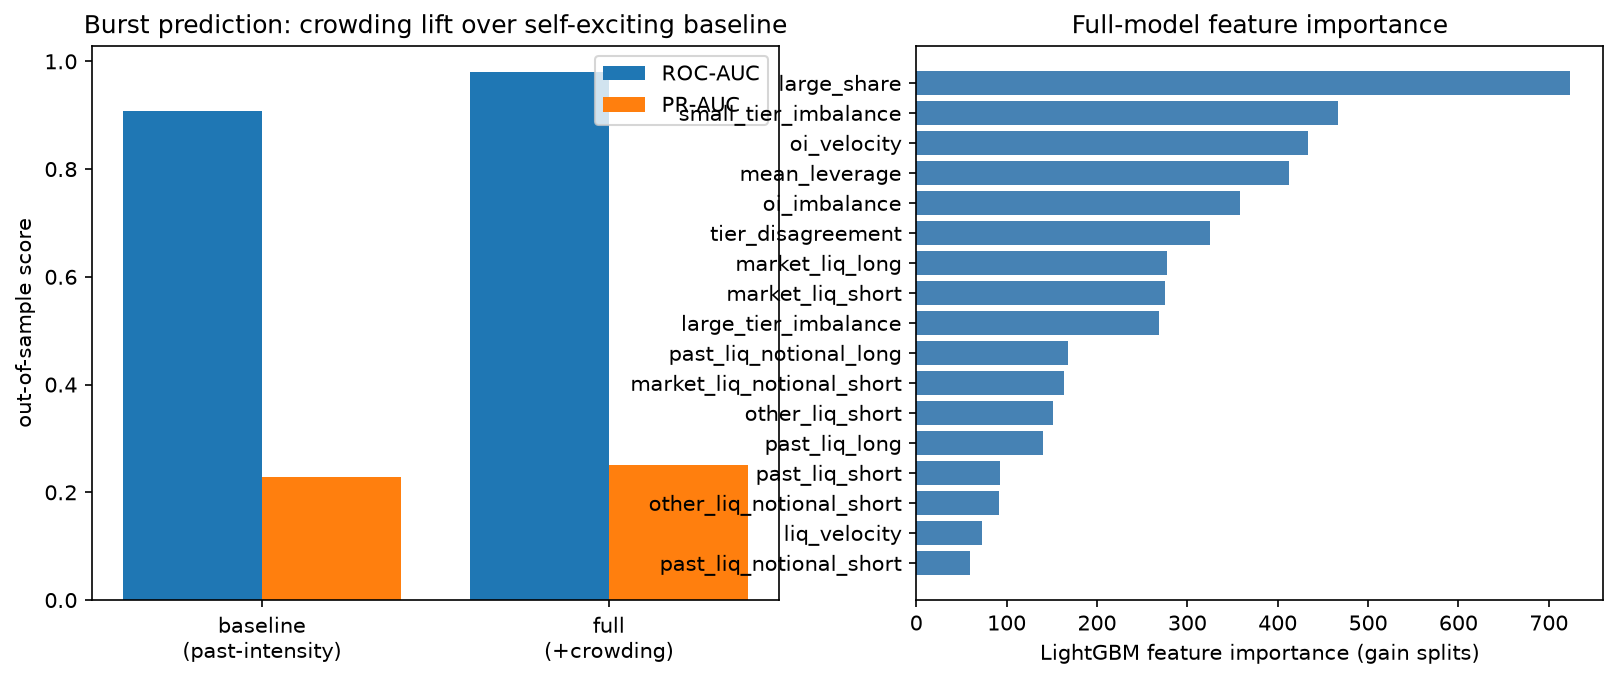
\includegraphics[width=0.92\textwidth]{../pipeline/outputs/b01_burst_baseline/burst_baseline_lift.png}
    \caption{Burst prediction on a leakage-safe, time-ordered test period. Left: out-of-sample ROC-AUC and PR-AUC for the self-exciting LightGBM baseline (past-intensity only) versus the tuned full model ($+$crowding$+$volume$+$cross-asset). Right: LightGBM feature importances of the full model, showing the relative contribution of the tier-crowding and cross-asset features over the trailing-intensity baseline. See Table~\ref{tab:m2} for the full comparison against the classical-Hawkes and neural-THP baselines.}
    \label{fig:m1}
\end{figure}

\paragraph{References.} Full BibTeX entries in \texttt{references.bib}; supporting probe reports in \texttt{m0-magnet-findings.md}, \texttt{m0-burst-findings.md}, \texttt{m1-crowding-lift-findings.md}, \texttt{m2-baselines-findings.md}. Key works: Bacry, Mastromatteo \& Muzy (2015, Hawkes in finance); Hardiman, Bercot \& Bouchaud (2013, branching-ratio Hawkes); Filimonov \& Sornette (2012, reflexivity / flash crashes); Cao \& Palaash (2025, multivariate-Hawkes DeFi liquidations); Zuo et al.\ (2020, Transformer Hawkes Process); Mei \& Eisner (2017, Neural Hawkes Process); Du et al.\ (2016, recurrent marked TPP); Xue et al.\ (2023, EasyTPP benchmark); Gibbs \& Cand\`es (2021) and Zaffran et al.\ (2022, adaptive conformal prediction).

\end{document}
